\section{Data Preprocessing}
Here we discuss how to process the Beijing dataset. The overall process is illustrated in \ref{fig:data-processing}. 
\begin{figure}[h!]
  \centering
    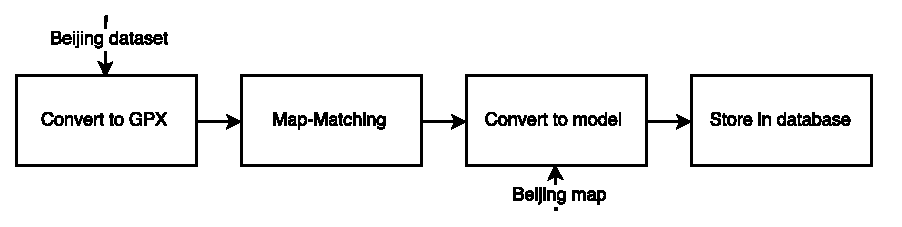
\includegraphics[width=1\textwidth]{figures/data-processing.pdf}
    \caption{From raw gps data to database}
    \label{fig:data-processing}
\end{figure}
The gps dataset is converted into the GPX format which is subsequently map-matched to the road network of Beijing. The map-matched data is then converted into the model objects of the system, and are then stored in the respective tables of the database. Likewise, the map of the Beijing road network is converted to model objects and stored in the database. By doing so, we have a knowledge base of the road network of Beijing and data about vehicle movements in a unified format. \todo{maybe we should perform some data cleaning}
\subsection{Map generation}
To model the road network of Beijing we need to have the specific information about all the roads in the road network. This information is available several places, but most of these services are not free. We have chosen to work with OpenStreetMap which is an open source map service, where users collaborate to keep the city maps updated. There are some problems in using this kind of service, such as the possibility of wrong data, limited data, etc\todo{Er det godt nok bare at skrive etc? + kilde?}. But because this service was the only free service that we could find, we see no other option than having in mind that these problems can occur. We have also found that OpenStreetMap cannot export large areas of a map, such as the whole city of Beijing. Therefore we have chosen to use one of its mirror sites, Geofabrik, which holds extract\todo{Forstår ikke helt det?} of the whole world, segmented into countries and these are updated daily. This makes it possible for us to extract the whole map for China.

\subsubsection{Format \& Pre-processing}
The maps from Geofabrik comes in a compressed format called pbf. To extract the relevant data from this format we are using a tool called Osmosis, to query the file using several filters to be able to extract only the information relevant.
We are using two types of filters with Osmosis, the first is to limit the area that we want to extract, since the map we got is for all of China. The second filter is used to extract only roads from the restricted area.
With this filter we have the possibility to specify which roads we want to have in the output. Because all paths are marked in OpenStreetMap as a way, we want to filter paths such as side-walks, bicycle ways, and other ways that are not possible to use with a car.

The extracted data from the Osmosis query is then exported to a file which is structured in a way that resembles the XML format. There are two types left in the export, which are nodes and ways. Nodes represent road intersections and are also used to indicate points along a road if the road is curved. Both nodes and ways can include key-value pairs that contain information, i.e. if a way is one-way, if a intersection have a traffic light, ect\todo{igen, er etc godt nok at skrive?}.
Ways are almost similar structured, but they also contain a nd tag which contains a value the id of a node related to the way.\todo{Forstår ikke den sidste sætning her}

\begin{lstlisting}[style=XML, caption=Node representation]
<node id, version, timestamp, uid, user, changeset, longitude, latitude >
	<tag key, value />
</node>
\end{lstlisting}

\begin{lstlisting}[style=XML, caption=Way representation]
<Way id, version, timestamp, uid, user, changeset >
	<nd ref />
	<tag key, value />
</way>
\end{lstlisting}

We have illustrated the representation of nodes, ways, edges and segments in \figref{fig:waywithnodes}. Where the red nodes are intersections, the green nodes are points along a way, ways are the black lines, edges are the lines between every node, and a segment is the blue lines between intersection nodes.

\begin{figure}[h!]
  \centering
    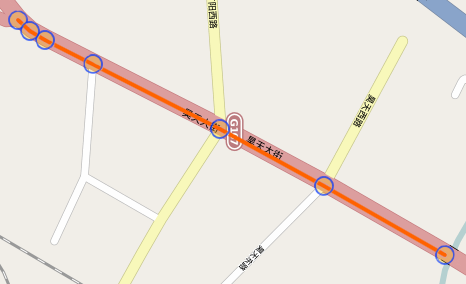
\includegraphics[width=0.8\textwidth]{figures/way-w-nodes.png}
    \caption{A way with nodes}
    \label{fig:waywithnodes}
\end{figure}

\subsubsection{Generation}
To be able to extract the information in the Osmosis export, a XML parser is used to model the road network. When a node or way tag is read a equivalent data structure is created and stored. 
\begin{lstlisting}[style=java, caption=Datastructure for a node]
Node{
	long id;
	double longitude;
	double latitude;
	Ways[] connectedWays;
}
\end{lstlisting}

\begin{lstlisting}[style=java, caption=Datastructure for a way]
Way{
	long id;
	Node[] connectedNodes;
	int type;
}
\end{lstlisting}

We want to model the road network as a graph, but the relation between ways and nodes are not in this format when exported from Osmosis, so we have to work on the data structures generated from the parser.
Besides the original way and node data structures, we have chosen to create two other classes such that we are able to construct a graph, these are called edges and segments.
Edges are the links between every two nodes and a segment is the link between to intersection nodes. When generating these classes from ways and nodes, we have to check whether a way has a tag attached to it which describes if the way is one-way or not, because if it is we have to create edges and segments in both directions.

\begin{lstlisting}[style=java, caption=Datastructure for an edge]
Edge{
	long id;
	double length;
	long origin;
	long destination;
	long segment;
}
\end{lstlisting}

\begin{lstlisting}[style=java, caption=Datastructure for a segment]
Segment{
	long id;
	double length;
	long way;
	long origin;
	long destination;
}
\end{lstlisting}

The relation between edges and segments is that each edge of a segment contains a reference to the segment that it is a part of, the same is true from the relation between ways and segments.
\subsection{Data cleaning}
\begin{itemize}
\item removal of gps coordinates outside city limits.
\item normalising huge speeds to speed limit. / removing speeds.
\end{itemize}

\subsection{Map matching}
The Beijing dataset consists timestamped samples of gps-coordinates. The format of the samples is (id, date time, longitude, latitude). However since GPS measurements can be inaccurate, it is not always possible to directly infer which road the sample was taken on. Consequently the coordinates must be map-matched to a road, such that positions on the road can be inferred. To perform map-matching, the system calls the TrackMatching webservice\cite{TrackMatching}. This service exposes an API for map-matching to the OpenStreetMap service and given a dataset of raw GPS-coordinates returns a map-matched dataset in JSON format. 
\todo{write about how and why map generation}
\todo{write about how and why we design DB and store data in SQL database}